\chapter{Forord}
I denne rapport dokumenterer vi vores valg i forhold til implementationen af opgaverne i Obligatorisk opgave 2.

Kildekode og testdokumentation kan findes i appendix på side \pageref{Appendix}. Vores git repository kan findes på https://github.com/esfdk/BOSC/tree/master/oo2.

Vi ville gerne have lavet mere fyldestgørende test af opgave 4.

\chapter{Beskrivelse af implementation}
\section{Opgave 1}
\label{O1}
Vi skal optimere en sekvensiel funktion, der udregner summen af kvadratrødder, således at den kører hurtigere på en multicore maskine end den ellers ville have gjort. Dette skal gøres ved hjælp af tråde.

Koden til funktionen kan findes i 'mul\_sum/mulsum.c'. Den er løst baseret på koden fra Operating System Concepts, 8th edition, side 161.

\subsection{Del 1}
\label{O1_1}
\begin{my_itemize}
\item Udregning af hvilke tal hver tråd skal arbejde med.
\item Lav tråde med oprettede structs.
\item Udregning af sum af kvadratrødder.
\item Resultat af alle tråde.
\end{my_itemize}
\paragraph{Arbejde} Før vi opretter vores tråde, udregner vi hvor mange tal hver tråd skal arbejde med. Derefter laver vi en beregning til at finde de laveste og højeste tal. Det gør vi blandet andet ved "double minnum = floor(work * n) + 1;". Vi bruger floor, da vi kun er intersseret i heltal. Når det er gjort, opretter vi struct og placerer dem i arrays såsom "calc\_result[n].minimum\_number = minnum;" (se linje 44-52). 
\paragraph{Oprettelse af tråde} Når vi har fundet ud af hvilket arbejdet hver tråd skal udføre, opretter vi dem. Hver tråd bliver sat til at køre TaskCode med et struct fra punkt 1 som parameter (se linje 57-60).
\paragraph{Udregning} Derefter laver vi selve udregningen, hvor vi finder summen af kvadratrødderne. Når en tråd er færdig med sin del, bliver der kaldt pthread\_exit på den, hvilket får den til at terminere (se linje 17-29).
\paragraph{Beregning af resultat} For at finde det samlede resultat går vi igennem arrayet af structs og tilgår deres sumsqrt værdi. Alle disse værdier ligger vi sammen og printer dem ud (se linje 71-75).

\subsection{Del 2}
\label{O1_2}
I opgave 1.2 bliver vi bedt om at tjekke vores multitrådet sum-funktion vha. en speedup graf.
En speedup graf viser hvor meget hurtigere en funktion bliver, når man lader arbejdet foregå på flere tråde.

\begin{figure}[h!]
\centering
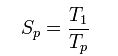
\includegraphics{Images/oo2-1-2-SpeedUpFormel}
\caption{Formel til udregning af speedup}
\label{SpeedFormel}
\end{figure}

Speedup udregnes ved at tage kørselstiden ved 1 tråd og dividere det med kørselstiden med n tråde, som i vores tilfælde er 1, 2, 4, 6 og 8. Det optimale resultat ville være en linær speedup, hvor speedupen er lig antallet af tråde, som funktionen er blevet kørt med.

\begin{figure}[h!]
\centering
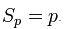
\includegraphics{Images/oo2-1-2-IdealSpeedUp}
\caption{Ideal speedup}
\label{IdealSpeed}
\end{figure}

\paragraph{Valg af maskine til speedupgraf}
Til test af vores multitrådet sum-funktion havde vi valget mellem to eller fire processore eller fire processor med hyperthreading. Vi valgte at bruge computeren med fire processor. Det gjorde vi fordi det var medianen og vi mente,  det var hvad en standard computer ville have. Dette ville give os nogle mere generelle resultater. 

\subparagraph{Uventet resultat ved kørsel med fire tråde}

\begin{figure}[h!]
\centering
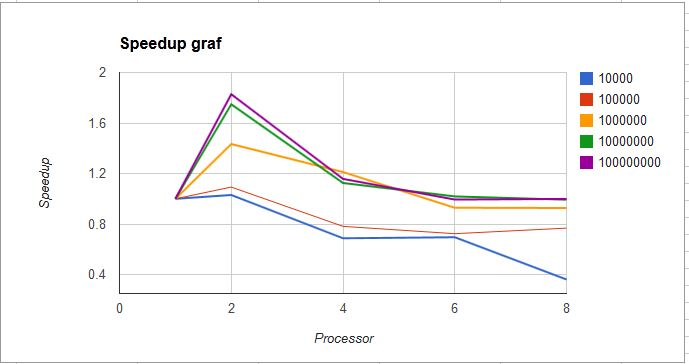
\includegraphics{Images/oo2-1-2-FrederikSpeedUp}
\caption{Speedup graf for maskine med 4 processors}
\label{FrederikSpeed}
\end{figure}

Som man kan se udfra vores speedup graf, er der næsten en ideal speedup fra en tråd til to tråde. Ved fire tråde bliver den dog kun en smule hurtigere end ved en tråd. Dette resultat synes vi er fovirrende, da det burde være muligt at få en speedup svarende til speeduppen fra en tråd til to tråde. Computeren har trods alt fire realle processor. Vi har ingen forklaring på hvorfor det er sådan. 
Vi havde forventet at få problemer ved seks og otte tråde da vi ikke har mulighed for at tildele hver tråd en processer. 

\begin{figure}[h!]
\centering
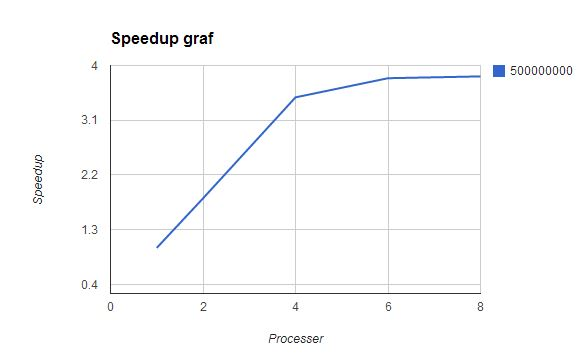
\includegraphics{Images/oo2-1-2-MelnykSpeedUp}
\caption{Speedup graf for maskine med 4 processors og hyper-threading}
\label{MelnykSpeed}
\end{figure}

Vi har kort testet vores funktion på en laptop med fire processor og hyperthreading, hvor vi havde en normal speedup optil fire tråde. Dette er forståligt da fire processor med hyperthreading kun 'simulerer' otte processor, og derfor ikke arbejder ligeså optimalt som otte konkrete processor.

\subsection{Tests}
\label{O1_Tests}
For at teste om vores forbedret multitrådet sum-funktion kørte hurtigere med flere tråde, brugte vi en speedupgraf som nævnt i \ref{O1_2}. For at lave en ordenlig speedupgraf lavede vi 10 runs af funktionen ved 1-2-4-6-8 tråde ved input 10.000. Input blev gjort 10 gange højere per iteration op til 100.000.000 samt fra 50.000 og så gjort 10 gange højere op per iteration til 500.000.000. Dette gjorde, at vi havde en stor mængde data til at lave en graf over gennemsnittet af vores timings.

Vores resultater kan findes både i appendix \ref{Speedup_Output} på side \pageref{Speedup_Output} og GoogleDocs på bitly.com/U0EYAK

\section{Opgave 2}
\label{O2}
Vores løsning af opgave 2 er beskrevet i 'FIFO/list.c' og 'FIFO/list.h'. Testkoden til listen er beskrevet i 'FIFO/testNoThreads.c' og 'FIFO/tetstThreads.c'. 'list.c', 'list.h' og 'testNoThreads.c' er baseret på kode fra 'opg2' zip-filen fra bloggen\footnote{https://blog.itu.dk/BOSC-E2012/files/2012/10/opg2.zip}.
\subsection{Del 1}
\label{O2_1}
Vi har valgt at implementere 'list\_add(List *l, Node *n)' på en meget simpel måde (se linje 35 til 41 i list.c). Listens sidste element ('l-\textgreater last') bliver sat til at pege på den nye node ('l-\textgreater last-\textgreater next = n'), hvorefter 'l-\textgreater last' bliver sat til at være n. På denne måde vil det anden sidste element pege på det nye element, og 'last' peger på det nye element, da det er det sidste i listen.
\\'*list\_remove(List *l)' implementationen kan ses på linje 44 til 60 i list.c filen. I funktionen bliver der lavet en 'Node *n'. Denne node bliver sat til at være det første element i listen, altså 'l-\textgreater first-\textgreater next' da 'first' er root elementet og aldrig skal pilles ved. Rodelementets 'next' bliver sat til at pege på n's 'next', hvilket er det andet element i listen. På denne måde er det første element blevet "fjernet" fra listen. Funktionen tjekker derefter om 'first-\textgreater next' er null, for hvis den er, skal 'last' pege på først, ligesom da listen lige var blevet lavet. Til slut retuneres n.

\subsection{Del 2}
\label{O2_2}
Det mest åbenlyse problem er, at flere tråde kan editere listen på samme tid. For eksempel: To tråde tilgør listen på samme tid og finder frem til det sidste element ('last'). Begge tråde prøver at tilføje et element til listen, hvilket betyder at de begge prøver at tilføje et element til 'last' på samme tid. Tråd \#1 tilføjer sit element til 'last', hvorefter tråd \#2 tilføjer sit element til 'last' (det element som \#1 lige har tilføjet sit element til), hvilket ødelægger linket mellem 'last' og tråd \#1s element.

En anden udgave af problemet ovenover er, hvis to forskellige tråde vil remove på samme tid. Tråd \#1 går ind og læser 'first's 'next' element (da det skal blive first efter removal). Samtidig går tråd \#2 ind og kører hele removal, hvorefter \#1 prøver at fjerne det element der lige er blevet fjernet. Derved er kun et element blevet fjernet, hvor to elementer burde have været fjernet. Den omvendte situation kan også opstå, hvor to elementer bliver fjernet, men hver tråd tror kun at et element er blevet fjernet.

Alt efter størrelsen af listen kan der også opstå problemet. Hvis listen kun er et element langt og en tråd prøver at adde mens en anden prøver at remove, kan der opstå forkerte resultater. Sker de samtidig, kan elementet blive addet (hvilket gør at listen er to elementer lang), på samme tid som det første (og eneste) element bliver removet. Risikoen er, at det nye element bliver appendet på det element der lige er blevet removet, hvorved ingen af elementerne er i listen.

\subsection{Del 3}
\label{O2_3}
Vi har brugt mutex låse i list\_add og list\_remove funktionerne. I list\_add er de to linjer logik inde i en mutex lock, da det ikke skal være muligt for flere tråde, at tilføje elementer på samme tid. I list\_remove er alt undtagen return-statementet indkapslet af mutex locks af samme årsag som i list\_add; det skal ikke være mulgit at fjerne flere elementer samtidig. At 'return n' ikke er i en lock, gør dog ingen skade. Når funktionen når til 'return', bruger den ikke listen mere, og det kan derfor køres uden at være i en lock.
Vi har beskrevet vores test at den flertrådet liste i afsnit \ref{O2_Tests}.

\subsection{Tests}
\label{O2_Tests}
Vi har lavet to tests til first-in-first-out listen. En test uden brug af tråde for at se om lsiten overhovedet virker, og en test med tråde, for at sikre at flere tråde kan bruge listen samtidig, uden der opstår problemer.
\\Testen uden brug at tråde findes i testNoThreads.c. I denne test laver vi en liste, tilføjer to elementer til listen, fjerner to elementer fra listen og printer deres værdier for at sikre os, at de er kommet ud i den rigtige rækkefølge. 
\\Testen med tråde findes i testThreads.c og er lidt mere omfattende. Testen tager to parametre: Antallet af tråde der skal laves, og antallet af elementer hver tråd skal håndtere. 'main' funktionen laver et array med det valgte antal tråde, og sætter dem alle samme til at køre '*TaskCode(void *argument)' funktionen. Hver tråd får sit eget nummer i arrayet med, for at man nemmere kan holde styr på hvilken tråd der gør hvad. Hver tråd laver det valgte antal elementer (som er strings med formatet ("Thread \#\%d, element \%d", threadNumber, elementNumber)) og adder dem til listen. Derefter fjerner tråden det antal elementer, som den har addet til listen og printer værdien af disse elementer. 
\\Det man kan se med testThreads testen er, at trådene går ind og låser listen når de bruger den. Som oftest vil elementerne være i rækkefølge, så det er alle tråd \#1's elementer først, så tråd \#2's, osv.

\section{Opgave 3}
\label{O3}
Vores løsning af opgave 3 er beskrevet i 'prod\_cons/prodCons.c' samt 'prod\_cons/prodCons.h'. 'prod\_cons/List' mappen indeholer vores list fra opgave 2, som vi også inkluderer i 'FIFO'-mappen.

I denne opgave har vi brugt 'pthread\_mutex\_t' objekter til at undgå problemer hvor flere tråde ændrer samme element på samme tid. 'pthread\_mutex\_t' er objekter, der kan låses/låses op via 'pthread\_mutex\_lock'-funktions kaldet. Hvis en funktion låser en mutex, forhindre den derved andre funktioner i at køre videre, forudsat at de selv skal bruge mutex'en. De andre funktioner går i stå indtil mutex'en låses op igen, hvilket sørger for, at critical code kun køres af en tråd ad gangen. Bruger man ikke mutex låse i et flertrådet program, risikerer man at løbe ind i situationer hvor flere tråde har modificeret samme element på samme tid, hvilket kan ødelægge programmet.
\\ Vi har også brugt 'sem\_t' objekter, også kaldet semaphore. Det er objekter, der indeholder en værdi, og som kan bruges af funktioner til synkronisation mellem tråde. De har to interessante funktioner: 'sem\_wait(sem\_t)' og 'sem\_post(sem\_t)'. 'sem\_wait()' kigger på værdien af semaphoren. Hvis værdien er mindre end nul, vil den kaldende funktion pause, og vente på værdien bliver højere end nul. Når det sker, vil den kaldende funktion få lov til at køre videre og 'sem\_wait()' reducerer værdien af semaphoren med en. 'sem\_post()' forøger simpelthen bare værdien af semaphoren med en.
\\ Både 'phtread\_mutex\_t' og 'sem\_t' objekter virker som låse, omend på forskellige måder. 'pthread\_mutex\_t' virker som en ja/nej, og vil kun lade en tråd udføre sit arbejde ad gangen. 'sem\_t' lader gerne flere tråde arbejde på samme tid, så længe semaphorens værdi er over nul.

\subsection{Opfyldelse af punkter}
\label{O3_Punkter}
\paragraph{Punkt 1} - Vores implementation gør det muligt at definere antallet af producers, antallet af consumers, størrelsen på bufferen og antallet af produkter der skal produceres. Dette gør vi, ved først at tjekke om der er den rigtige mænge inputs, hvorefter vi konveterer inputs til ints og bruger dem til at lave de forskellige ting (se linje 36-48).
\paragraph{Punkt 2} - Punkt 2 opfyldes af koden. Vi har kun en producer funktion og en consumer funktion (henholdsvis linje 120 og 160), og consumer/producer tråde laves og sættes til at køre det respektive kode (se linje 84-104).
\paragraph{Punkt 3} - Både producer funktionen og consumer funktionen kalder 'sleepRandom' funktionen hver gang de udfører deres logik (se linje 155 og 188), som sætter tråden til at sove i et tilfældigt antal sekunder (se linje 214-221).
\paragraph{Punkt 4} - Vi sørger for at tråde ikke udsultes ved at lade tråde sove i et tilfældigt antal sekunder, når de har arbejdet. På denne måde forhindrer vi tråde i at tage alle opgaverne og derved udsult andre tråde.
\paragraph{Punkt 5} - Se afsnit \ref{O3_Output} i Appendix for output.
\paragraph{Punkt 6} - Vi opfylder dette krav igennem et tjek i starten af både consumer og producer funktionerne. I starten af producer funktionen, tjekkes der om der stadig skal produceres flere produkter. Hvis der ikke skal, afsluttes producer tråden. Consumeren tjekker, om der er konsumeret lige så mange produkter som skulle produceres. Hvis der er, afsluttes consumer tråden.
\subsection{Tests}
\label{O3_Tests}

\section{Opgave 4}
\label{O4}
Vores løsning af opgave 4 er beskrevet i 'bankeralgorithm/banker.c' samt i appendix. Den er baseret på den ufuldstændige banker.c fra zip-filen\footnote{https://blog.itu.dk/BOSC-E2012/files/2012/10/banker.zip} på kursusbloggen.

I forhold til beskrivelsen af Banker's algoritmen i Operating System Concepts, 8th edition, så er m og n byttet om, således at i vores kode er 'm' antallet af processer og 'n' er antallet af resurser.

\subsection{Opfyldelse af punkter}
\label{O4_Punkter}
\paragraph{Punkt 1} - Vi allokerer memory til state dynamisk ved bruge af malloc. Dette gør vi efter at antallet af processer og resurser er blevet læst ind. Vi var nødt til at inkludere et for-loop, da 'max', 'allocation' og 'need' er "arrays of pointers to arrays".  (Se linje 226-238).
\\I slutningen af 'main()' funktionen frigiver det memory, som vi har allocated til state. Vi gør dette i omvendt rækkefølge, da vi er nødt til at tilgå resurse arrays'ne før vi kan frigive processer arrays'ne. (Se linje 311-322).
\paragraph{Punkt 2} - Vi har implementeret safety algoritmen som beskrevet på side 299 i Operating System Concepts, 8th Edition. Vi initialiserer 'work' og 'finish' som beskrevet. Derefter har vi et while-loop, som kører step 2 og step 3 af algoritmen indtil der er en iteration, hvor der ikke er en process, hvis 'finish' status skifter til true(1). Dette gør vi, fordi det er ligegyldigt, i hvilken rækkefølge processerne bliver færdig i forhold til safe eller unsafe state. (Se linje 95-159).
\\I hvert kald til 'resource\_request(int i, int *request)' låser vi 'state\_mutex' således at state ikke tilgås af mere end en process. Herefter udfører vi første step af 'resource-request' algoritmen\footnote{Beskrevet på side 299 i Operating System Concepts, 8th edition.}. Hvis dette step fejler, så crasher vi programmet. Ellers går vi videre til step 2, hvor vi unlocker låsen og return 0, hvis requesten ikke kan opfyldes. 
\\Hvis requesten måske kan opfyldes, laver vi ændringerne til state og kalder vores 'safety\_check()' funktion. Hvis 'safety\_check()' er false, så laver vi rollback på state, releaser lock og returner 0. Ellers unlocker vi låsen, beholder vores ændringer til state og returner 1. (Se linje 32-78).
\paragraph{Punkt 3} - I 'resource\_release(int i, int *request)'  låser vi 'state\_mutex', så andre tråde ikke kan tilgå state og gør det modsatte af step 3 af 'resource-request' algoritmen. Herefter unlocker vi låsen og funktionen afslutter. (Se linje 81-92).
\paragraph{Punkt 4} - Efter state er blevet oprettet i 'main(int argc, char* argv[])', kalder vi 'safety\_check()'. Hvis det returner false, crasher vi, ellers forsætter. (Se linje 286-294).
\paragraph{Punkt 5} - Da vi locker 'state\_mutex' i 'resource\_request(int i, int *request)', 'resource\_release(int i, int *request)', 'generate\_request(int i, int *request)' og 'generate\_release(int i, int *request)' er der ikke flere tråde, som kan tilgå state på samme tid. 'safety\_check()' tilgår state, men den bliver kun kaldt inde i en block kode, hvor 'state\_mutex' er låst og i 'main(int argc, char* argv[])' før trådene bliver oprettet.

\subsection{Tests}
\label{O4_Tests}
Programmet kører og rapporterer, at begge de to eksempel input filer fra zip-filen fra kursusbloggen\footnote{https://blog.itu.dk/BOSC-E2012/files/2012/10/banker.zip} er safe. Hvis den første linje i 'allocation matrix' (matrix nr. 2 i  input filen) ændres fra '1 0 1' til '2 0 1', bliver den unsafe og dette rapporteres også korrekt.
\\Ellers har vi testet og set, at det ikke lader til, at programmet går i 'deadlock' eller lignende.
